\chapter{Mini Problems}

\section{Greatest Common Divisor}
\begin{exercise}
    Write a function to calculate the GCD of two integers.
    \begin{example}
        \label{ex:gcd:example1}
        \hfill \\
        Given $35$ and $28$ the function returns $7$.
    \end{example}
    
    \begin{example}
        \label{ex:gcd:example2}
        \hfill \\
        Given $15$ and $8$ the function returns $1$.
    \end{example}

    \end{exercise}

\subsection{\CC Brute-force}
The GCD of two numbers $x$ and $y$ is defined as the largest integer that divides both $x$ and $y$. A simple and inefficient solution would simply loop over all numbers from the smallest between $x$ and $y$ and would stop as soon as we find one that divides both. We are guaranteed to find such a nuber as the number $1$ will happily divide any number. This solution is shown in Listing \ref{list:gcd_bruteforce}.

\lstinputlisting[language=c++, caption={Brute-force, linear time solution.},label=list:gcd_bruteforce]{test/mini_problems/gcd/gcd_bruteforce.cpp}

\subsection{Log-time solution. Euclidean Algorithm}
A much faster solution can be achieved by using the Euclidean algorithm for the GCD.
This algorithm is based on the principle that the greatest common divisor of two numbers $x$ and $y$ does not change if the larger number is replaced by the reminder of the integral division between $x$ and $y$.

For example, $21$ is the GCD of $252$ and $105$ (as $252 = 21 \times 12$ and $105 = 21 \times 5$), and the same number $21$ is also the GCD of $105$ and $252 \mod 105 = 42$.
Since this replacement reduces the larger of the two numbers, repeating this process gives successively smaller pairs of numbers until we reach a point where the smallest numbers divides the largest and therefore the reminder is zero (in the worst case the smallest becomes $1$). 

It was proven by Gabriel Lamé in 1844 that this algorithm always terminates in less steps than five times the number of digits of the smaller number (in base 10) making this algorithm extremely efficient as the number of digits grows logaritmically compared the number it represents.

Listing \ref{list:gcd_euclide} shows a recursive implementation of this algorithm while Listing \ref{list:gcd_euclide_iterative} shows an iterative one. 

\lstinputlisting[language=c++, caption={Euclide algorithm, recursive implementation.},label=list:gcd_euclide]{test/mini_problems/gcd/gcd_euclide.cpp}

\lstinputlisting[language=c++, caption={Euclide algorithm, iterative implementation.},label=list:gcd_euclide_iterative]{test/mini_problems/gcd/gcd_euclide_iterative.cpp}

\subsection{\CC Compile-time}
It is quite common to see specific requirements on the compile implementation of the GCD algorithm. Therefore in this section we will see how we can calculate the GCD in \CC at compile time. 

Before C++-11 the only way to do compile time computation was by using templates. In order to calculate GCD using templates we will use a structure with two integral template parameters that we will manipulate in a \inline{static const} variable. An implementation of this idea is shown in \ref{list:gcd_euclide_precpp11}.

\lstinputlisting[language=c++, caption={Pre C++11, compile-time template based solution.},label=list:gcd_euclide_precpp11]{test/mini_problems/gcd/gcd_euclide_pre_cpp11.cpp}

The code works by have a template class with two integral template parameters and a partial specialization that is used to terminate the recursion which is triggered whenever we request the static field \inline{::gcd}.

C++-11 introduces \inline{constexpr} function that can be used to specify function that can be run at compile-time. In C++-11 there are quite some limitation in what statements and operations we can do in a \inline{constexpr} context: for instance we can only have one return statement. Most of these contraints are related in the subsequent versions of the standard. A \inline{constexpr} recursive solution that works in C++-11 is shown in Listing \ref{list:gcd_euclide_cpp11}.

\lstinputlisting[language=c++, caption={C++11 \inline{constexpr} based solution.},label=list:gcd_euclide_cpp11]{test/mini_problems/gcd/gcd_euclide_cpp11.cpp}

Notice that, from C++-14 we can decorate Listing \ref{list:gcd_euclide_iterative} with \inline{constexpr} so that it can be used in compile-time computation.



%%%%%%%%%%%%%%%%%%%%%%%%%%%%%%%%%%%%%%%%%%%%%%%%%%%%%%%%%%%

\section{Maximum Depth of N-ary Tree}
\begin{exercise}
   Given a N-ary tree, return its depth which is defined as the length of the longest path from the tree's root to any of its leaves.
    \begin{example}
        \label{ex:nary-treedepth:example1}
        \hfill \\
        Given the tree depicted in Figure \ref{fig:longest_consecutive_sequence:example1} the function returns $3$ (path from node $1$ to node $12$).
    \end{example}
    
    \begin{example}
        \label{ex:nary-treedepth:example2}
        \hfill \\
        Given the tree depicted in Figure \ref{fig:longest_consecutive_sequence:example2} the function returns $6$ (path from node $1$ to node $40$).
    \end{example}
    \end{exercise}
 
 
\begin{figure}
	\centering
	\begin{subfigure}[]{0.45\textwidth}
		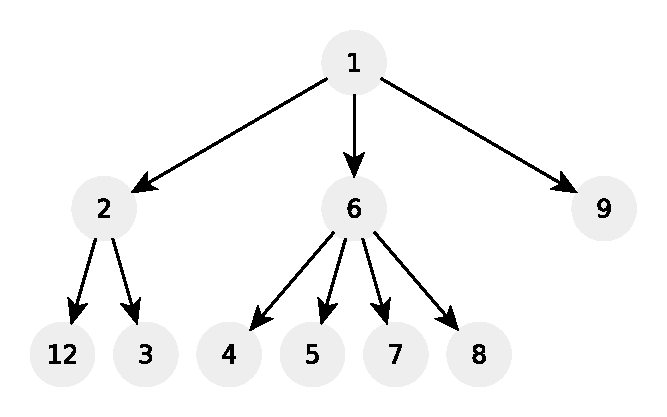
\includegraphics[width=1\linewidth]{sources/mini_problems/n-ary-tree-depth/images/example1}
		\caption{Input tree for Example \ref{ex:nary-treedepth:example1}.}
		\label{fig:longest_consecutive_sequence:example1}
	 \end{subfigure}
	\hfill
	\begin{subfigure}[]{0.45\textwidth}
		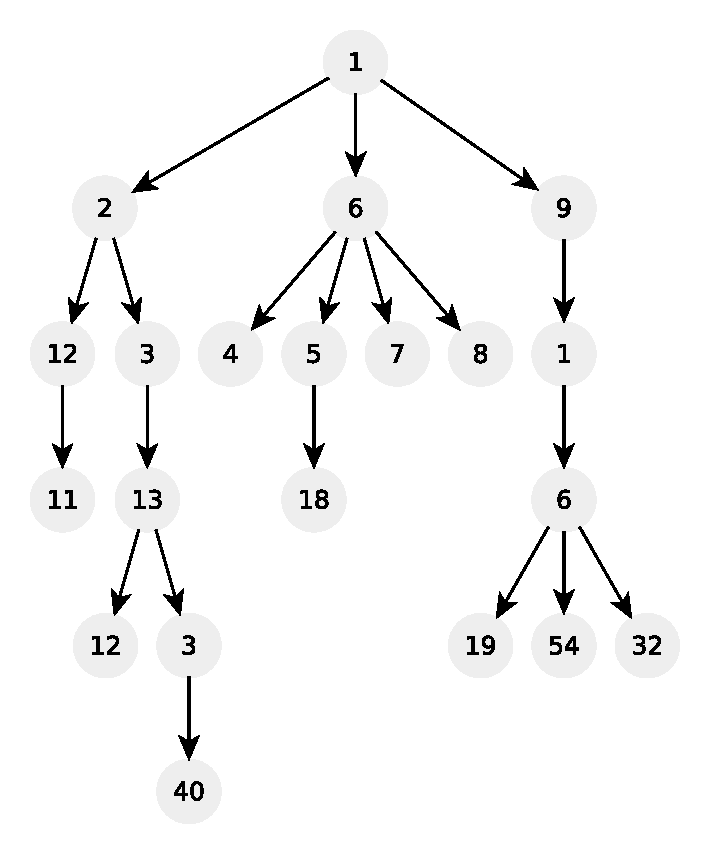
\includegraphics[width=1\linewidth]{sources/mini_problems/n-ary-tree-depth/images/example2}
		\caption{Input tree for Example \ref{ex:nary-treedepth:example2}.}
		\label{fig:longest_consecutive_sequence:example1}
	 \end{subfigure}
	 \caption[]{}
	  \label{}
\end{figure}
    
\subsection{Discussion}
    This is a classical problem, mostly asked during phone screening due to its simplicity. 
    What the problem, in other words, is asking us to do, is to return the maximum level of any of the tree's nodes.
    The level of a node is the number of its ancestors plus one. 
    Therefore to solve this problem, all we have to do is to visit the tree and keep track of the number of ancestors which is equivalent to the number of steps down the tree we took.
    We know that the root has $0$ ancestors and therefore, we know that each of its children will have $1$ ancestor (the root itself) and that any of its grandchildren will have $2$ ancestors and so on.
    
    Visiting a tree can be equally easily done recursively and iteratively as shown in Sections \ref{} and \ref{}, respectively.
 
    For the reminder of the discussion, we will define the root of a tree to be a pointer to the \inline{Node} structure defined in Listing \ref{list:n-arytreedepth:nodedef}.
 
    \begin{lstlisting}[language=c++, caption={Node definition.},label=list:n-arytreedepth:nodedef]]{
class Node {
public:
    int val;
    vector<Node*> children;

    Node() {}

    Node(int _val) {
        val = _val;
    }

    Node(int _val, vector<Node*> _children) {
        val = _val;
        children = _children;
    }
};            
    \end{lstlisting} 
    

\subsection{Recursive solution}
The recursive solution has the advantage of being shorter in terms of lines of code and in our opinion more elegant. It could, however, underperform the iterative solution if the compiler is not able to optimize the code properly or lead to out of memory errors if the tree depth goes over a certain value because at any given time, we keep in the stack a number of activation records that is equal to the level of the node we are visiting.

Listing \ref{list:n-ary-treedepth_recursive}  shows an implementation of this approach and has a linear time and space (considering the space occupied by the activation records) in the number of nodes of the tree.

\lstinputlisting[language=c++, caption={Recursive solution.},label=list:n-ary-treedepth_recursive]{test/mini_problems/n-ary-treedepth/n-ary-treedepth_recursive.cpp}

\subsection{Iterative Solution}
The same idea can be implemented iteratively as shown in Listing \ref{list:n-ary-treedepth_iterative} where we use a stack to keep track of the nodes \textbf{and their level}. Whenever we visit a node, we compare its level with the maximum found so far, then we remove it from the stack and insert all of its children in the stack with a level value increased by one. 

\lstinputlisting[language=c++, caption={Iterative solution.},label=list:n-ary-treedepth_iterative]{test/mini_problems/n-ary-treedepth/n-ary-treedepth_iterative.cpp}


%%%%%%%%%%%%%%%%%%%%%%%%%%%%%%%%%%%%%%%%%%%%%%%%%%%%%%%%%%%

\section{Assigning cookies \faCookie}
\begin{exercise}
    You are the parent of $n$ children and you want to make them happy by giving them a cookies (real ones  \faCookieBite, not HTTP cookie). 
    However you know that too many cookied are not good for them and therefore you settle for a rule that each child can at most get one cookie.
    Giving cookies to your children is not easy as they are special and each child $i$ has an integer greed factor $g[i]$ associated,
    which is the minimum size of a cookie that the child $i$ will be content with; 
    You have at your disposal a number $m$ of cookies, and each cookie $j$ has an integer size $s[j]$.
    You can give cookie number $i$ to child number $i$ if and only if $s[j] \ge g[i]$. When a child has a cookie assigned is content.
    
    Write a function that given a list  ($G$) of $n$ greed values and a list ($C$) of  $m$ cookie sizes determines the maximum possible of children you can make content.
     
    \begin{example}
        \label{ex:nary-treedepth:example1}
        \hfill \\
        Given $G=\{1,2,3\}$ and  $=\{1,1\}$ the function returns $1$. Despite having two cookies we can only make one child happy because we do not have cookies big enough for children number $2$ and $3$.
    \end{example}
    
    \begin{example}
        \label{ex:nary-treedepth:example2}
        \hfill \\
        Given $G=\{1,3\}$ and  $=\{1,4\}$ the function returns $2$. We can give the first cookie to the first child and the second cookie to the second child.
    \end{example}


    \begin{example}
        \label{ex:nary-treedepth:example3}
        \hfill \\
        Given $G=\{1,2,3\}$ and  $=\{1,1,3\}$ the function returns $2$. We can give the first cookie to the first child and the the third cookie to the second child The second cookie remains unassigned and the third child without cookie assigned.
    \end{example}
    \end{exercise}
 

\subsection{Discussion}
Let's start by noticing that despite what shown in the Exmaples the input lists are not guaranteed to be sorted and that, sorting actually makes solving this problem much easier.
The idea is that we have to find a way to assign to each children the smallest cookie possible that has size higher or equal to his greed. If the input array is not sorted then for each greed value we are forced to search $S$ entirely for a suitable cookie. 
If on the other hand both $G$ and $S$ are sorted then, we can try to accomodate children by increasing greed and keep track and assign progressively larger cookies to them. 
If a children with greed $i$ can be assigned cookie number $j$, then we can try to assign to child number $i+1$ cookie number $j+1$. If that does not work then we can try with cookie number $j+2$ and so on.
When we cannot assign a cookie $j$ to a certain child $i$, cookie $j$ will be unused, but that is not an issue because there is no way we can assign cookie $j$ to any other children because the greed values for children $i+1, i+2, \ldots$  will all be greater than the gree of child $i$.

Therefore in order to solve this problem we can:
\begin{itemize}
    \item sort $G$;
    \item sort $S$;
    \item use two pointers to keep track of the current child and current cookie
    \item process one child a the time until we ran out of children or cookies
    \item if the current cookie size is greater than the current child greed then we can advance both pointers
    \item otherwise we can only hope the next cookie will be assignable and therefore only advance the cookie pointer.
\end{itemize}

An implementation of this idea is shown in Listing \ref{list:assign_cookies_sorting}. Its time complexity is $O(nlog(n))$ while its the space complexity is $O(1)$.


\lstinputlisting[language=c++, caption={Solution using sorting.},label=list:assign_cookies_sorting]{test/mini_problems/assign_cookies/assign_cookies_sorting.cpp}


%%%%%%%%%%%%%%%%%%%%%%%%%%%%%%%%%%%%%%%%%%%%%%%%%%%%%%%%%%%

\section{Maximize Sum Of Array After K Negations}
\begin{exercise}
    Given an integer array $nums$ and an integer $k$, modify the array in the following way: choose an index $i$ and replace $nums[i]$ with $-nums[i]$.
    
    You should apply this process \textbf{exactly} $k$ times. You may choose the same index $i$ multiple times.
    
    Return the largest possible sum of all the elements of $nums$ at end of this process.     
    \begin{example}
        \label{ex:nary-treedepth:example1}
        \hfill \\
        Given $nums=\{4,2,3\}$ and $k=1$ the function returns $5$. We can choose index $1$ and turn the $2$ into $-2$. At the end we will be left with $nums=\{4,-2,3\}$ which totals to $4-2+3=5$.
    \end{example}
    
    \begin{example}
        \label{ex:nary-treedepth:example2}
        \hfill \\
        Given $nums=\{3,-1,0,2\}$ and $k=3$ the function returns $6$. We can choose 
    \end{example}


    \end{exercise}
 

\subsection{Discussion}
One easy way of solving this problem relies on the fact that all we have to do is to apply the change sign change always on the smallest number of the array.
The intuition behind it is that we should aim at first changing the sign of all the negative numbers first and among them we should prioritize the smallest ones: the number with the largest absolute value and negative sign. Changing the sign of those number will bring the best increase in the overall sum of the array.

If after having changed all negatives into positive we are left with more moved to make then we still have to change the sign of the smallest number in the array as many times as necessary.
This causes the smallest number of the array to switch sign back and forth until $k=0$ (this step can be optimized by noticing that if the number of moves left is even then the final valud of the smallest number in the array is not going to change, otherwise, it will be negative.We can reach this conclusion without having to actually perform the sign switch). 

To always keep track of the smallest number we can use a \inline{std::priority_queue} as shown in Listing \ref{}.

\lstinputlisting[language=c++, caption={Solution using sorting.},label=list:assign_cookies_sorting]{test/mini_problems/max_sum_array_after_k_negations/max_sum_array_after_k_negotiation_priority_queue.cpp}

The code works by applying the $k$ modifications always to the smallest element of the queue. At the end of the process we simply sum every element in the queue to obtain the answer. The complexity of this approach is $O(klog(n) + nlog(n))$ in time and $O(1)$ in space.


%%%%%%%%%%%%%%%%%%%%%%%%%%%%%%%%%%%%%%%%%%%%%%%%%%%%%%%%%%%

\section{Pairs of Songs With Total Durations Divisible by $k$}
\begin{exercise}
    You are given a list $T$ of songs where the $i^{th}$ song has a duration of $time[i]$ seconds.
    Write a function that given $T$ returns the number of distinct unordered pairs of songs for which the sum of their durations is divisible by an integer $k$.
    
    In other words,  the function should count the number of indices of $i < j$ such that $(T[i] + T[j]) \mod 60 == 0$.

     
    \begin{example}
        \label{ex:song_total_duration:example1}
        \hfill \\
        Given $T=\{30,20,150,100,40\}$ and $k=60$, the function returns $3$.
        We can pair songs at indices:
        \begin{itemize}
            \item $0$ and $2$ for a total duration of $180$;
             \item $1$ and $3$ for a total duration of $120$;
             \item $1$ and $4$ for a total duration of $60$.
        \end{itemize}
    \end{example}
    
    \end{exercise}
 

\subsection{Discussion}
This problem is quite similar to the two number sum problem discussed in Chapter \ref{ch:two_numbers_sum} and we will therefore use the very same technique to solve it (we will avoid discussing sub=optimal solution as the these are discussed already in the two number sum problem).
The difference here is that we are only interested in the number modulo $k$ and out main goal is to find two numbers whose remainder sum up to $0$.
For instance w.r.t. Example \ref{ex:song_total_duration:example1} we can see that  $T[0]+T[2] = 180$ which is divisible by $60$. 
If we have a look at their modulos are we notice that: $(T[0] \mod{60}) +(T[2] \mod{60}) = 30+30 = 60 \mod{60} =0$.
The same holds for the other two pairs of this example:
\begin{itemize}
    \item $(T[1] \mod{60}) +(T[3] \mod{60}) = 20+40 = 60 \mod{60} =0$
    \item $(T[1] \mod{60}) +(T[4] \mod{60}) = 20+40 = 60 \mod{60} =0$
\end{itemize}


Listing \ref{list:song_total_duration:lineartimespace} shows an implementation of this idea.

\lstinputlisting[language=c++, caption={Solution based on the two number sum problem.},label=list:song_total_duration:lineartimespace]{test/mini_problems/song_total_duration/song_total_duration_linear_time_space.cpp}


%%%%%%%%%%%%%%%%%%%%%%%%%%%%%%%%%%%%%%%%%%%%%%%%%%%%%%%%%%%

\section{Trim text}
\begin{exercise}
You are given a string $m$ of length $n$ and an integer $k$. $m$ is guaranteed to consists only of English alphabet letters and spaces.
Write a function that crops $s$ so that it becomes of lenght smaller or equal than $k$. However the cropped messages cannot:
\begin{itemize}
    \item crop away part of a word;
    \item have trailing spaces;
    \item have length greater than $k$;
\end{itemize}
Moreover the cropped string should be as long as possible i.e. any other cropped message satisfying the contraints above should be smaller than the output of your function.

     
    \begin{example}
        \label{ex:trim_text:example1}
        \hfill \\
        Given the input string \underline{\texttt{Lorem ipsum dolor sit amet\textvisiblespace }} and $k=6$ the function returns \underline{\texttt{Lorem}}.
        If $k=20$ the function returns \underline{\texttt{Lorem ipsum dolor}}.
        
        When if for instance $k=2$ or $k=3$ the function returns an empty string.
    \end{example}
    
\end{exercise}
 

\subsection{Discussion}
This problem on strings is all about implementation and there is no algorithmic insight that we need to have to solve it efficiently. 
However, this does not automatically make this problem an easy one as implementation-focused problems are often hard to get right. 
However, this specific problem can be tackled quite efficiently if we notice that we can remove characters from the back of $s$ if:
\begin{itemize}
    \item they are spaces, regardless of whether the current size of the string (the original string size minus the characters removed so far) is less than $k$;
    \item they are alphanumeric and the current length is strictly greater than $k$.
\end{itemize}
In particular, we can notice that we can safely remove trailing space from the original input as the problem statement clearly states that we cannot return a string with any of them.
Moreover, when we remove alphanumeric characters from the back of the string we are doing it only because the current size of $s$ is still strictly larger than $k$. 
When this happens we must remove all of these characters up until we reach a space. This is because we are forced not to crop away parts of words and we have to either keep a word o remove it entirely.

Listing \ref{list:trim_text:lineartime} shows an implementation of this idea.

\lstinputlisting[language=c++, caption={Linear time solution.},label=list:trim_text:lineartime]{test/mini_problems/trim_text/trim_text_solution1.cpp}

The function \inline{skip} is used to update the variable \inline{pos}, which is an index in \inline{s}. \inline{pos} keeps track of the portion of the input string we have not yet cropped.  
\inline{skip} moves \inline{pos} backwards until the user-provided function \inline{fn} returns true (and we have not reached the left limit of $s$).
\inline{skip} is used by the main driver function \inline{trim_text_lineartime} which is a function that repeatedly removes any trailing spaces and then, if the length of $s$ is still too large, proceed in removing an entire word. 
The word is also (like for spaces) removed by the function \inline{skip} which takes care of removing any character until it reaches the first non-alphanumeric character which we are assured to be a space (there are no other characters allowed in $s$).

The complexity of this approach is linear in time and constant in space (if we do not consider the space necessary for the output).


%%%%%%%%%%%%%%%%%%%%%%%%%%%%%%%%%%%%%%%%%%%%%%%%%%%%%%%%%%%

\section{Items and bags}
\begin{exercise}
A food bank is developing a system to help reduce its usage of plastic bags. The bank collects food from people that bring it in plastic bags. 
A plastic bag has a certain capacity $c$, which indicates the amount of food we can fit in it. In particular, a bag with a capacity $c$ can carry up to $c$ unit of goods.
The goal of the system is to rearrange the food in the warehouse into as few bags as possible to help reduce the waste footprint.

You are given two arrays $F$ and $B$ each consisting of $N$ integers where $F[i]$ is the amount of food currently present in the bag $i$ that has capacity specified in $F[i]$.
Write a function that returns the minimum number of bags needed to carry all food.

Notice that you are guaranteed $B[i] \geq F[i]$ to always hold.
    \begin{example}
        \label{ex:items_and_bags:example1}
        \hfill \\
        Given $F=\{1,4,1\}$ and $B=\{,1,5,1\}$ the funcion returns $2$. We could move $1$ unit of food from bag $0$ and put it in the bag $1$ (that currently holds $4$ units of food but has capacity $5$).
    \end{example}
    
    \begin{example}
        \label{ex:items_and_bags:example2}
        \hfill \\
        Given $F=\{2,3,4,2\}$ and $B=\{2,5,7,2\}$ the funcion returns $2$. All food in the bag $0$ can be moved to bag $1$ and all the food in bag $3$ can go in bag $2$.
    \end{example}
\end{exercise}
 

\subsection{Discussion}
This problem can be quickly solved with a greedy approach if we realize that we have a total amount of food units equal to $T=\sum F[i]$ that needs to fit into a subset of the $N$ bags we have at our disposal. 
The optimal arrangement is to fill the bags to their maximum capacity to avoid waste of space and to minimize the number of bags used we better use larger bags firsts as we can stuff more food units in them. 
Therefore, all we have to do to solve this problem is to sort the bags by capacity in descending order (larger bags first) and to simulate the process of filling them up until all the units of food are stored.

W.r.t to example \ref{ex:items_and_bags:example2}: we have $T=11$ units of food. If we put the first $7$ into the bag $2$ we are left with $T=11-7$ units of food not yet inside a bag. The next biggest bag is the one at index $1$ with a capacity of $5$. This bag can store all the $T$ units of food left. At this point, we can stop the simulation and return $2$.

Listing \ref{list:items_and_bags:solution1} shows an implementation of this idea.

\lstinputlisting[language=c++, caption={Solution based on sorting.},label=list:items_and_bags:solution1]{test/mini_problems/items_and_bags/items_and_bags_solution1.cpp}

The code works by first sorting $B$ in descending order and calculating the total amount of units of food we must store. Notice that we use \inline{std::accumulate} to perform this task instead of an explicit raw loop as it is more idiomatic and expressive.
The while loop takes care of performing the simulation, and each iteration tries to fill as much food as possible into a bag. The simulation stops when all food is safely inside a bag. 
Notice that we access \inline{B} using the variable \inline{Bidx} without checking that \inline{Bidx < B.size()} as the problem statement clearly states that there is always enough space among all bags to store all food. Therefore the while loop is guaranteed to put all food inside a bag before we ran out of bags.

The complexity of this approach is $O(Nlog(N))$ due to sorting while the space complexity is $O(1)$.

%%%%%%%%%%%%%%%%%%%%%%%%%%%%%%%%%%%%%%%%%%%%%%%%%%%%%%%%%%%

\section{Coupons}
\begin{exercise}
You want to buy $n$ item from Amazon. Their prices is stored in an array $P$ where $P[i] \geq 0$ contains the price for the item $i$. Amazon offers you the possibility to apply coupons to each item before the checkout and this causes the price of that item to halve.
For instance, if the full price of an item is 4.60\$, then after applying the coupons it costs $2.30\$$. You can apply coupons to an item multiple times, this means that if you apply the coupon three times to an item with price X\$, its final price will be $\frac{\frac{\frac{X}{2}}{2}}{2} = \frac{X}{2^3}$.
Your task is to write a function that calculates the minimum number of coupons needed in order to lower the cumulative checkout price for all of the $n$ items by half. 

    \begin{example}
        \label{ex:coupons:example1}
        \hfill \\
        Given $P=\{5,19,8,1\}$ the function should return $3$.  Initially the cart price is $5+19+8+1=33$. By applying two coupons to the item at index $1$ the price lowers to $5+\frac{19}{4}+8+1 = 18.75$ which is still higher than $\frac{33}{2}=16.5$. We can apply a third coupon to the item at index $0$ and the total price becomes $\frac{5}{2}+\frac{19}{4}+8+1 = 16.25$ which is good enough. 
    \end{example}
    
\end{exercise}
 

\subsection{Discussion}
When applying a coupon to an item with price $X$ we are going to save $\frac{X}{2}$ from its original price. If we only had one coupon to use, we would naturally apply it to the most expensive item as this will yield the biggest saving. We can extend this reasoning to $n$ coupons and apply the $n^{th}$ coupon to the most expensive item after having used $n-1$ coupons. 
To solve this problem we can simulate the process of applying coupons. As we use the coupons we must keep track of the item in the cart with the highest price, to which we can apply the coupon. We repeat this process until the amount of money saved is higher than half of the original cart price. 

A \inline{priority_queue} can be used to keep track of the most expensive item in the cart.

Listing \ref{list:coupons:solution1} implements this idea.

\lstinputlisting[language=c++, caption={Priority-queue basedvsolution.},label=list:coupons:solution1]{test/mini_problems/coupons/coupons_solution1.cpp}

The code works by creating a \inline{priority_queue} where prices are sorted in descending order. It is initialized with the prices in $P$.
The while loop continuously pop elements from the top of the queue, calculate the amount of money saved by applying the coupon to the popped-out element, and adds the halved prices back into the queue.

If it is not difficult to show that the while loop runs at most $n$ times as if we half the price of each element in $P$, we will as a consequence also halve $\sum P[i]$ (the original cart price). 
Therefore the time complexity is $O(nlog(n))$ (remember that operations on the queue are $O(log(n))$). The space complexity is $O(n)$ due to the space required by the priority queue itself.


%%%%%%%%%%%%%%%%%%%%%%%%%%%%%%%%%%%%%%
% Count comforming bitmask
%%%%%%%%%%%%%%%%%%%%%%%%%%%%%%%%%%%%%%
%!TEX root = ../main.tex
%%%%%%%%%%%%%%%%%%%%%%%%%%%%%%%%%%
% Links:
%
% Difficulty:
% Companies: 
%%%%%%%%%%%%%%%%%%%%%%%%%%%%%%%%%%


%\begin{figure}
%	\centering
%	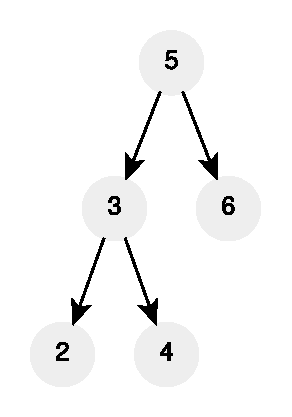
\includegraphics[width=\textwidth]{sources/count_numbers_conforming_bitmask/images/example1}
%	\caption[Sample short cpation]{Sample Caption}.
%	\label{fig:count_numbers_conforming_bitmask:example1}
%\end{figure}

\section{Count number integer conforming to any of the bitmasks}
\label{ch:count_numbers_conforming_bitmask}

\section{Problem statement}
\begin{exercise}
\label{example:count_numbers_conforming_bitmask:exercice1}
In this problem we consider unsigned 30-bit integers, i.e. all integers in the range $0,2^{30}$.
We say that integer $A$ conforms to integer $B$ if, in all positions where $B$ has bits set to $1$, $A$ has corresponding bits set to $1$.

For example $$00 0000 1111 0111 1101 1110 0000 1111 = 16244239$$ conforms to $$00 0000 1100 0110 1101 1110 0000 0001 = 13032961$$ while $$11 0000 1101 0111 0000 1010 0000 0101 = 819399173$$ does not conform to $$00 0000 1001 0110 0011 0011 0000 1111 =9843741$$

Write a function that given three 30-bit unsigned integers $A,B,C$ returns the number of unsigned 30-bit integers conforming to any among $A,B,C$.

	%example1
	\begin{example}
		\label{example:count_numbers_conforming_bitmask:example1}
		\hfill \\
		Given $$A = 11 1111 1111 1111 1111 1111 1001 1111 = 1073741727$$
		$$B = 11 1111 1111 1111 1111 1111 0011 1111 = 1073741631$$
		$$C = 11 1111 1111 1111 1111 1111 0110 1111 = 1073741679$$
		the function returns $8$. The following are the $8$ numbers comforming to $A$ or $B$ or $C$.
		\begin{itemize}
			\item  $11 1111 1111 1111 1111 1111 0011 1111 = 1073741631$
			\item  $11 1111 1111 1111 1111 1111 0110 1111 = 1073741679$
			\item  $11 1111 1111 1111 1111 1111 0111 1111 = 1073741695$
			\item  $11 1111 1111 1111 1111 1111 1001 1111 = 1073741727$
			\item  $11 1111 1111 1111 1111 1111 1011 1111 = 1073741759$
			\item  $11 1111 1111 1111 1111 1111 1101 1111 = 1073741791$
			\item  $11 1111 1111 1111 1111 1111 1110 1111 = 1073741807$
			\item  $11 1111 1111 1111 1111 1111 1111 1111 = 1073741823$
		\end{itemize}

	\end{example}

\end{exercise}


\section{Discussion}
\label{count_numbers_conforming_bitmask:sec:discussion}
Let's start by solving an easier version of this problem by trying to answer the following question: how many numbers are conformant to exactly a given unsigned $A$?
We know for sure that an integer $x$ must have its bit number $i$ set if $A$ bit number $i$ is set as well. However for every bit in $A$  that is \textbf{not} set we have a free choice between setting it or not. 
Because we have two choices for each of these positions, the total number of conformant number to $A$ is $2^{z}$ where $z$ is the number of bits not set in $A$.
For instance there are exactly $4$ numbers that are conformat to $11 1111 1111 1111 1111 1111 0101 1111$ as we have two choices for the bit at index $5$ and two choices for the bit at index $7$.

What about the numbers that are simultaneusly conformat to two numbers $A$ and $B$? In order for an unsigned to be conformat to both it must be the case that $x$ has its bit at position $i$ set if either the bit at position $i$ in $A$ or $B$ is set (or in both).
If the bit at position $i$ is set in $A$ but not set in $B$, the bit at position $i$ in $x$ must still be set in order for it to be conformat to both $A$ and $B$, and we can see that the same is true if the bit at position $i$ is set in $B$ and not set in $A$ or when it is set in both $A$ and $B$. Regardless of the case, it must be set in $x$ if any between $A$ and $B$ has it set.
Now, we can extend this reasoning and say that a number $x$ is conformat to several numbers $A$,$B$,$C\ldots$ simultaneusly if $x$ is conformant to $A \: \vee \: B \: \vee C \:  \vee \: \ldots$ (where $\vee$ symbolizes the bitwise OR operation).

We can use this fact and build a solution around it if we realize that we can count all numbers that are conformat to $A$, $B$ and $C$ separately and adds the results together as shown in Figure \ref{fig:count_numbers_conforming_bitmask:sets}. However by doing so we might count some numbers more than necessary and in particular, when adding together the number of numbers conformat to $A$ to the number of numbers conformat to $B$ we are counting the number of numbers conformat to $A$ \textbf{and} $B$ twice! The same reasoning applies for $A$ and $C$ and for $B$ and $C$ and for the number of numbers that are conformat to $A$, $B$ and $C$ simultaneusly. These are counted three times.

From Figure \ref{fig:count_numbers_conforming_bitmask:sets} it is easy to visualize how many times each intersections of the sets $A,B$ and $C$ is counted and from there visualize that the final answer is:
$$ |A \cup B \cup C| = |A|+|B|+|C| - |A \cup B| - |A \cup C| - |B \cup C| + |A \cup B \cup C|$$. 
This is basically the inclusion-exclusion principle at work which generalizes the familiar method for counting the number of elements in the union of two finite sets.


An implementation of this idea is shown in Listing \ref{list:count_numbers_conforming_bitmask:incexl}.

\begin{figure}
	\centering
	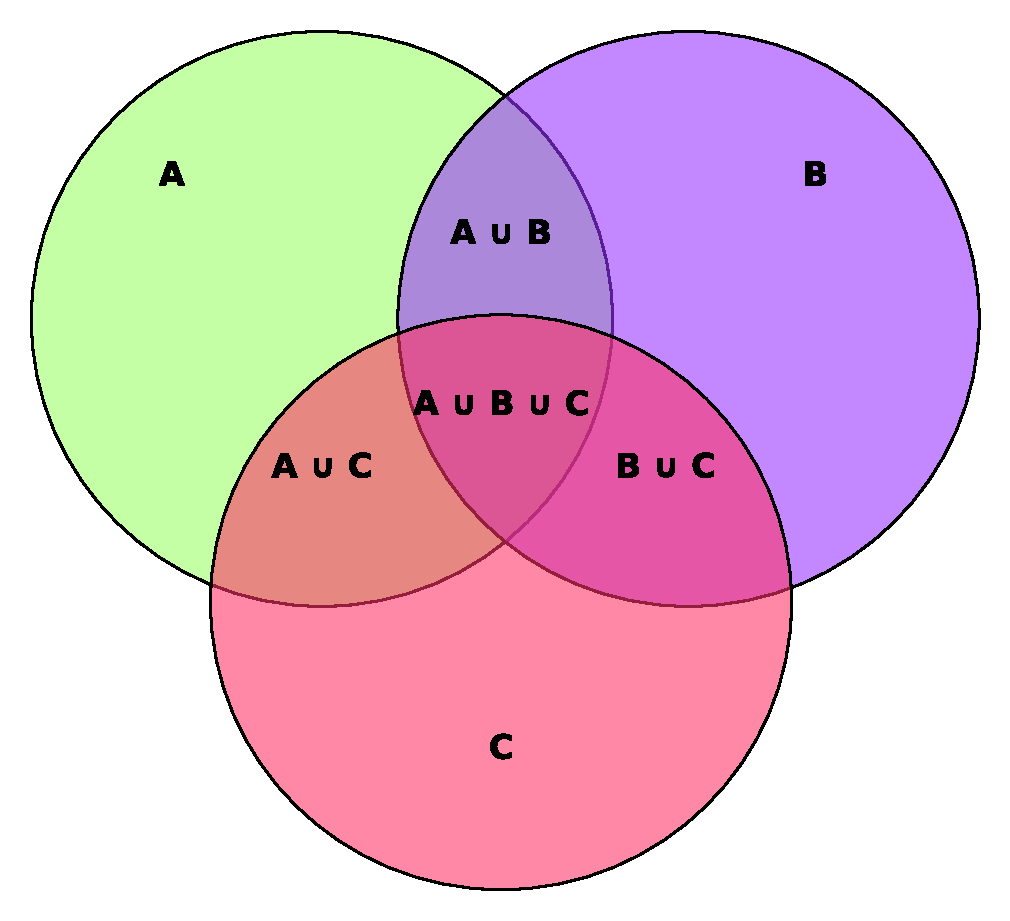
\includegraphics[width=\textwidth]{sources/count_numbers_conforming_bitmask/images/sets}
	\caption[Sample short cpation]{Sample Caption}.
	\label{fig:count_numbers_conforming_bitmask:sets}
\end{figure}

\subsection{Brute-force}
\label{count_numbers_conforming_bitmask:sec:bruteforce}

\lstinputlisting[language=c++, caption={Solution based on the inclusion-exclusion counting tecnique.},label=list:count_numbers_conforming_bitmask:incexl]{sources/count_numbers_conforming_bitmask/count_numbers_conforming_bitmask_solution1.cpp}

The function \inline{count_conforming} is responsible for counting the numbers conforming to just a single integer $N$ and it does so by counting the number of bit that are not set in $N$ which is equal to $30$ (the total number of bits in $N$) minus the number in $N$ that are set. To do so we use the function \inline{std::popcount} that is part of the \inline{<bit>} header is returns the number of $1$ bits in the argument (performs the same task as the GCC compiler intrinsic \inline{__builtin_popcount}).




%%%%%%%%%%%%%%%%%%%%%%%%%%%%%%%%%%%%%%
% Spiral matrix
%%%%%%%%%%%%%%%%%%%%%%%%%%%%%%%%%%%%%%
%!TEX root = ../main.tex
%%%%%%%%%%%%%%%%%%%%%%%%%%%%%%%%%%
% Links:
%
% Difficulty:
% Companies: 
%%%%%%%%%%%%%%%%%%%%%%%%%%%%%%%%%%


%\begin{figure}
%	\centering
%	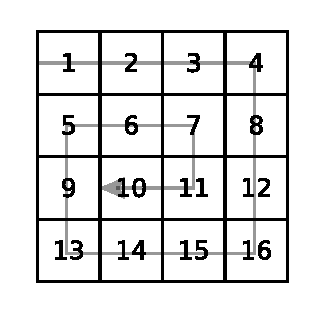
\includegraphics[width=\textwidth]{sources/spiral_matrix/images/example1}
%	\caption[Sample short cpation]{Sample Caption}.
%	\label{fig:spiral_matrix:example1}
%\end{figure}

\section{Spiral Matrix}
\label{ch:spiral_matrix}

\section{Problem statement}
Given a matrix $M$ of size $m\times n$ return a list containing the elements of $M$ in spiral order.
\begin{exercise}
\label{example:spiral_matrix:exercice1}

	%example1
	\begin{example}
		\label{example:spiral_matrix:example1}
		\hfill \\
		Given the matrix shown in Figure \ref{fig:spiral_matrix:example1}  the function returns \inline{1,2,3,4,5,6,7,8,9};
	
		
	\end{example}

	%example2
	\begin{example}
		\label{example:spiral_matrix:example2}
		\hfill \\
		Given the matrix shown in Figure \ref{fig:spiral_matrix:example2}  the function returns \inline{1,2,3,4,8,12,16,15,14,13,9,5,6,7,11,10};
	\end{example}

\end{exercise}
\begin{figure}[t]
    \centering
    \begin{subfigure}[]{0.45\textwidth}
        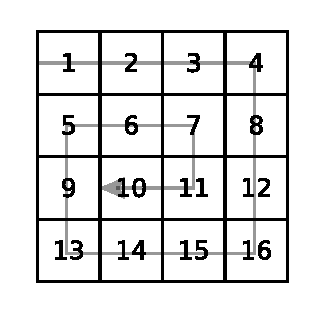
\includegraphics[width=\textwidth]{sources/spiral_matrix/images/example1}
        \caption[]{}
        \label{fig:spiral_matrix:example1}
     \end{subfigure}
    \hfill
    \begin{subfigure}[]{0.45\textwidth}
        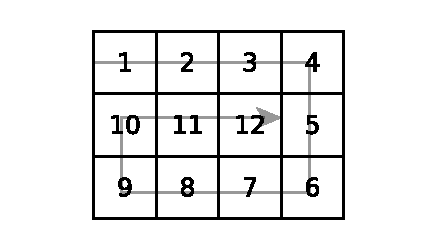
\includegraphics[width=\textwidth]{sources/spiral_matrix/images/example2}
        \caption[]{}
        \label{fig:spiral_matrix:example2}
    \end{subfigure}
\end{figure}



\section{Discussion}
\label{spiral_matrix:sec:discussion}


\subsection{Brute-force}
\label{spiral_matrix:sec:bruteforce}

	\lstinputlisting[language=c++, caption={Sample Caption},label=list:spiral_matrix]{sources/spiral_matrix/spiral_matrix_solution1.cpp}

